\documentclass[12pt]{elsarticle}
\usepackage[bottom=2cm,top=3cm,left=3cm,right=2cm]{geometry}
\usepackage{url}
\makeatletter
\def\ps@pprintTitle{%
      	\let\@oddhead\@empty
      	\let\@evenhead\@empty
      	\def\@oddfoot{\reset@font\hfil\thepage\hfil}
      	\let\@evenfoot\@oddfoot
}
\makeatother

\usepackage{babelbib}

\usepackage[brazilian]{babel} % Traduz alguns termos para o português
\usepackage[utf8]{inputenc} % Reconhece acentuação
\usepackage{setspace}

\onehalfspacing

\begin{document}

	\begin{frontmatter}

		\title{ELE083 Computação Evolucionária\\ \resizebox{7cm}{0.3cm}{Laboratório III - Evolução Diferencial}}
		\author{Davi Pinheiro Viana - 2013029912\\Rafael Carneiro de Castro - 2013030210}
		\address{Minas Gerais, Brasil}
		
		\begin{keyword}
			Computação Evolucionária\sep Evolução Diferencial
		\end{keyword}
	\end{frontmatter}
	
	\section{Introdução}
	O objetivo do trabalho é implementar o algoritmo da \emph{Evolução Diferencial (ED)} e utiliza-lo em dois problemas de otimização, para se avaliar seu desempenho e precisão. O algoritmo de Evolução Diferencial usa como mecanismo básico de busca o operador de mutação diferencial. É muito popular na otimização não linear com variáveis contínuas e é simples de implementar, robusto, versátil, autoadaptativo e eficiente.

	\section{O Algoritmo da Evolução Diferencial}
	A seguir, na Figura \ref{fig:pseudo-code}, pode ser visto o pseudo-código do algoritmo de evolução diferencial implementado neste trabalho.
	
	Este algoritmo foi implementa no MatLAB, e pode ser visto nos arquivos \textit{lab3\_peaks} e \textit{lab3\_rastrigin} anexos junto a este relatório.
	
	\section{Testando com as funções peaks e rastrigin}
	As funções \textit{peaks} e \textit{rastrigin} foram disponibilizadas e foram utilizadas para se testar o algoritmo da Evolução Diferencial. Para a função \textit{peaks}, as variáveis $x1$ e $x2$ estão ambas no intervalo $[-3; 3]$, e tem mínimo global em $f(x^*) = -6.5511$, onde $x^* = [0.228; -1.625]$. Já para a função \textit{rastrigin}, as variáveis $x1$ e $x2$ estão ambas no intervalo $[-2; 2]$, e tem mínimo global em $f(x^*) = -20$, onde $x^* = [0; 0]$. O algoritmo foi executado para a otimização de ambas as funções, e algumas iterações podem ser vistas nas Figuras \ref{fig:peaks} e \ref{fig:rastrigin}. O mínimo global da função peaks foi bem aproximado pelo algoritmo em estudo a partir da geração (iteração) 40. Já para a função rastrigin, o mínimo global foi bem aproximado a partir da geração 50.
	
	\pagebreak
	\begin{figure}[h]
		\centering
		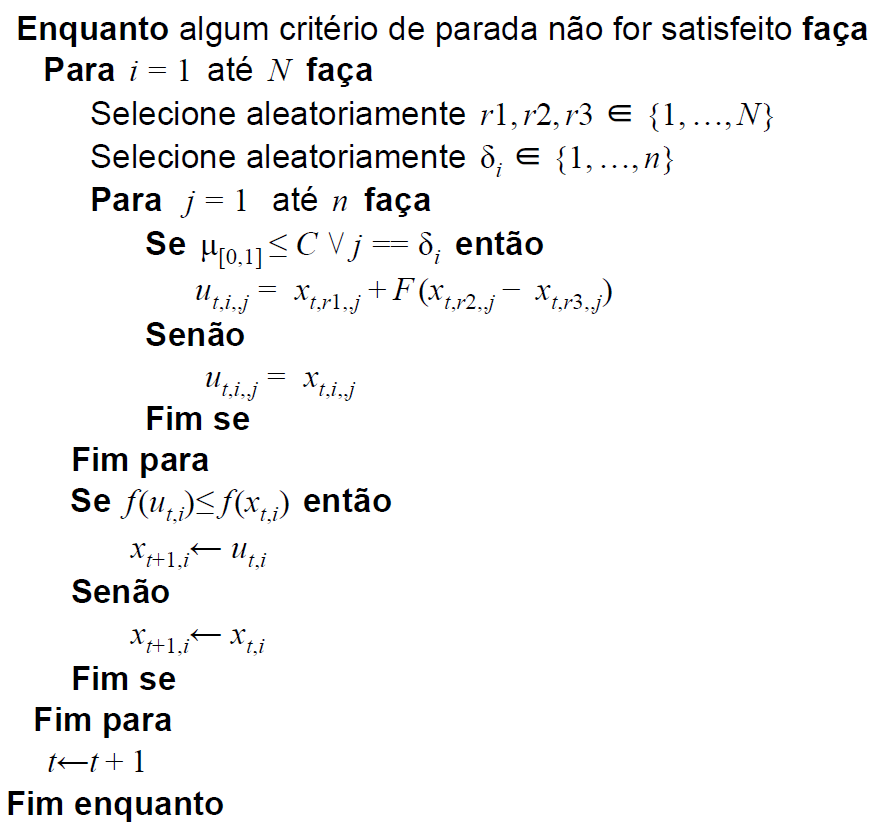
\includegraphics[width=10cm]{img/pseudo-code.png}
		\caption{Pseudo-código implementado}
		\label{fig:pseudo-code}
	\end{figure}
	\begin{figure}[h]
		\centering
		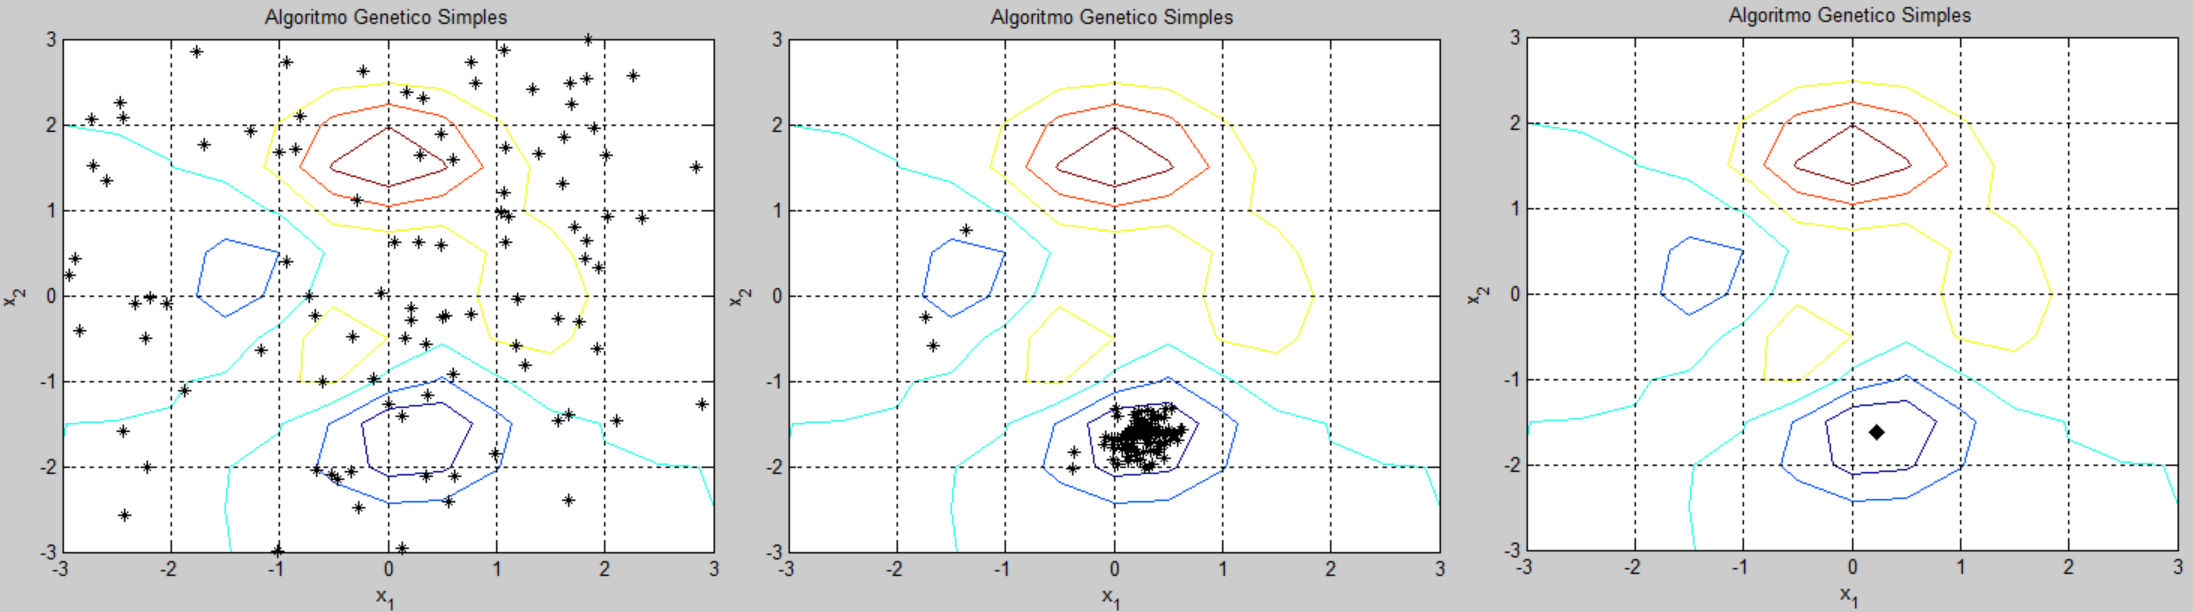
\includegraphics[width=17cm]{img/peaks.png}
		\caption{Interações do algoritmo para a função \textit{peaks} nas gerações 1, 20 e 40}
		\label{fig:peaks}
	\end{figure}
	\begin{figure}[h]
		\centering
		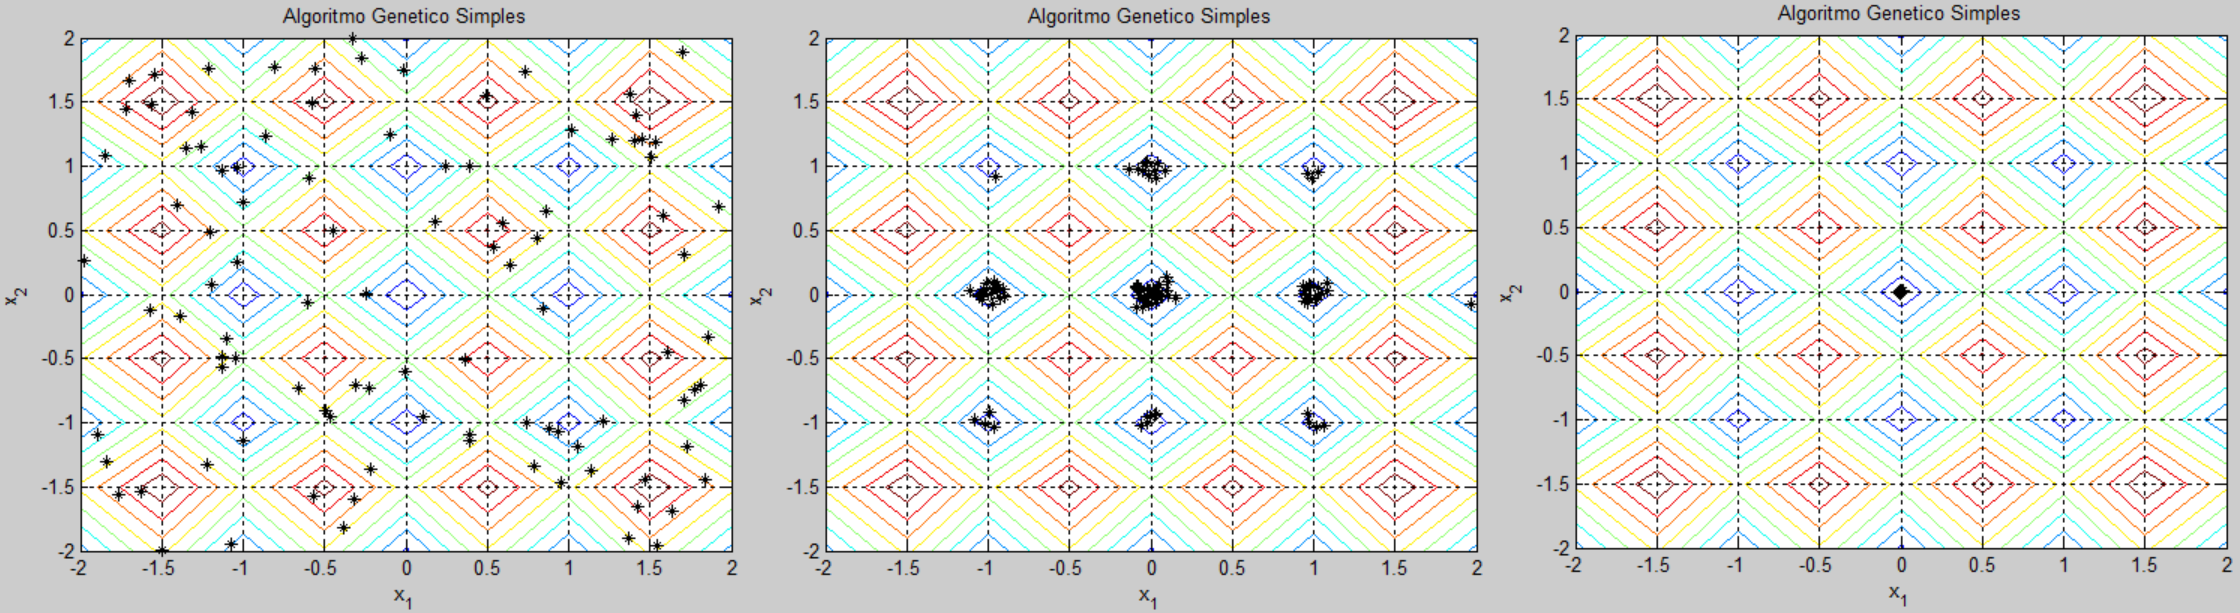
\includegraphics[width=17cm]{img/rastrigin.png}
		\caption{Interações do algoritmo para a função \textit{rastrigin} nas gerações 1, 25 e 50}
		\label{fig:rastrigin}
	\end{figure}
	
	\pagebreak
	\section{Conclusão}
	A partir dos resultados obtidos, pode-se concluir que para ambas as funções testadas o algoritmo da Evolução Diferencial obteve resultados bem precisos, e com relativamente poucas iterações do código. O algoritmo é bem intuitivo e foi de simples implementação. Conclui-se assim que os objetivos propostos pela tarefa foram cumpridos.
	
\end{document}